\documentclass{article}

% packages
\usepackage{amsmath, amsthm, thmtools, amsfonts, amssymb, luacode, catchfile, tikzducks, hyperref, ifthen}
\ifcsname c@kobocompile\endcsname
	\usepackage[a5paper, total={1072pt, 1448pt}, margin=10pt, includeheadfoot]{geometry} % set page margins
\else
	\usepackage[a4paper, margin=50pt, includeheadfoot]{geometry}
\fi
\usepackage[shortlabels]{enumitem}
\usepackage[skip=3pt, indent=0pt]{parskip}

% language
\usepackage[bidi=basic, layout=tabular, provide=*]{babel}
\ifcsname c@english\endcsname
	\babelprovide[main, import]{english}
\else
	\babelprovide[main, import]{hebrew}
	\babelprovide{rl}
\fi
%\babelfont{rm}{Libertinus Serif}
\babelfont{rm}[Renderer=Harfbuzz]{Libertinus Serif}
\babelfont{sf}{Libertinus Sans}
\babelfont{tt}{Libertinus Mono}

% style
\AddToHook{cmd/section/before}{\clearpage}	% Add line break before section
\linespread{1.3}
\setcounter{secnumdepth}{0}		% Remove default number tags from sections, this won't do well with theorems
\AtBeginDocument{\setlength{\belowdisplayskip}{3pt}}
\AtBeginDocument{\setlength{\abovedisplayskip}{3pt}}
\graphicspath{ {../images/} }

% operators
\DeclareMathOperator\cis{cis}
\DeclareMathOperator\Sp{Sp}
\DeclareMathOperator\tr{tr}
\DeclareMathOperator\im{Im}
\DeclareMathOperator\re{Re}
\DeclareMathOperator\diag{diag}
\DeclareMathOperator*\lowlim{\underline{lim}}
\DeclareMathOperator*\uplim{\overline{lim}}
\DeclareMathOperator\rng{rng}
\DeclareMathOperator\Sym{Sym}
\DeclareMathOperator\Arg{Arg}
\DeclareMathOperator\Log{Log}
\DeclareMathOperator\dom{dom}
\DeclareMathOperator\supp{Supp}
\DeclareMathOperator\var{Var}
\DeclareMathOperator\cov{Cov}

% commands
%\renewcommand\qedsymbol{\textbf{מש''ל}}
%\renewcommand\qedsymbol{\fbox{\emoji{lizard}}}
\newcommand{\Aa}[0]{\mathcal{A}}
\newcommand{\Bb}[0]{\mathcal{B}}
\newcommand{\CC}[0]{\mathbb{C}}
\newcommand{\Cc}[0]{\mathcal{C}}
\newcommand{\EE}[0]{\mathbb{E}}
\newcommand{\FF}[0]{\mathbb{F}}
\newcommand{\Ff}[0]{\mathcal{F}}
\newcommand{\Ii}[0]{\mathcal{I}}
\newcommand{\Gg}[0]{\mathcal{G}}
\newcommand{\Ll}[0]{\mathcal{L}}
\newcommand{\Mm}[0]{\mathcal{M}}
\newcommand{\NN}[0]{\mathbb{N}}
\newcommand{\Nn}[0]{\mathcal{N}}
\newcommand{\PP}[0]{\mathbb{P}}
\newcommand{\Pp}[0]{\mathcal{P}}
\newcommand{\QQ}[0]{\mathbb{Q}}
\newcommand{\RR}[0]{\mathbb{R}}
\newcommand{\Rr}[0]{\mathcal{R}}
\newcommand{\Ss}[0]{\mathcal{S}}
\newcommand{\TT}[0]{\mathbb{T}}
\newcommand{\Uu}[0]{\mathcal{U}}
\newcommand{\Vv}[0]{\mathcal{V}}
\newcommand{\Ww}[0]{\mathcal{W}}
\newcommand{\ZZ}[0]{\mathbb{Z}}
\newcommand{\acts}[0]{\circlearrowright}
\newcommand{\explain}[2] {
	\begin{flalign*}
		 && \text{#2} && \text{#1}
	\end{flalign*}
}
\newcommand{\maketitleprint}[0]{ \begin{center}
	%\begin{tikzpicture}[scale=3]
	%	\duck[graduate=gray!20!black, tassel=red!70!black]
	%\end{tikzpicture}	
	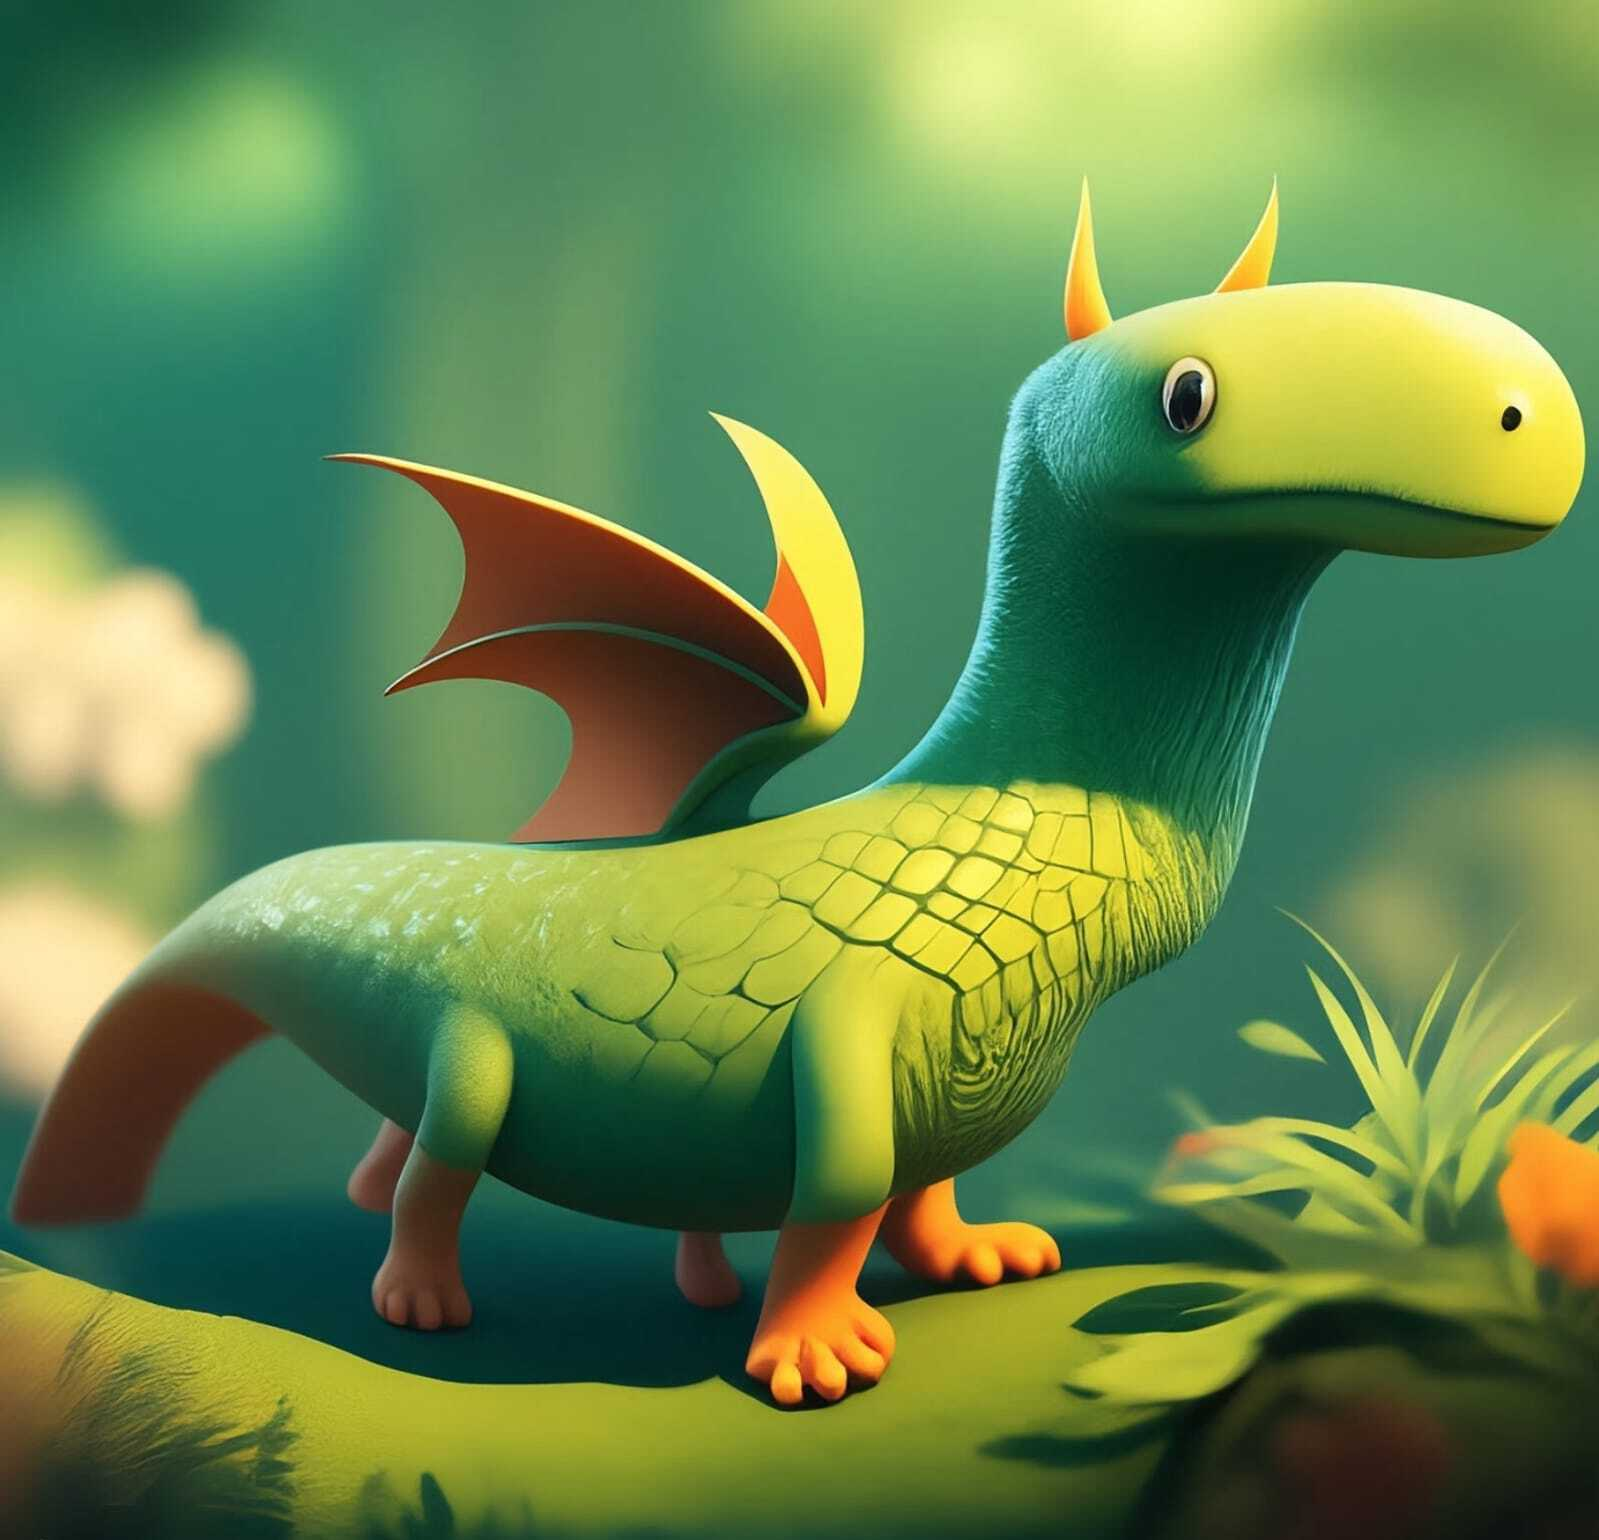
\includegraphics[width=6cm]{cover}
\end{center}
}

% theorem commands
\newtheoremstyle{c_remark}
	{}	% Space above
	{}	% Space below
	{}% Body font
	{}	% Indent amount
	{\bfseries}	% Theorem head font
	{}	% Punctuation after theorem head
	{.5em}	% Space after theorem head
	{\thmname{#1}\thmnumber{ #2}\thmnote{ \normalfont{\text{(#3)}}}}	% head content
\newtheoremstyle{c_definition}
	{3pt}	% Space above
	{3pt}	% Space below
	{}% Body font
	{}	% Indent amount
	{\bfseries}	% Theorem head font
	{}	% Punctuation after theorem head
	{.5em}	% Space after theorem head
	{\thmname{#1}\thmnumber{ #2}\thmnote{ \normalfont{\text{(#3)}}}}	% head content
\newtheoremstyle{c_plain}
	{3pt}	% Space above
	{3pt}	% Space below
	{\itshape}% Body font
	{}	% Indent amount
	{\bfseries}	% Theorem head font
	{}	% Punctuation after theorem head
	{.5em}	% Space after theorem head
	{\thmname{#1}\thmnumber{ #2}\thmnote{ \text{(#3)}}}	% head content

\ifcsname c@english\endcsname
	\theoremstyle{plain}
	\newtheorem{theorem}{Theorem}[section]
	\newtheorem{lemma}[theorem]{Lemma}
	\newtheorem{proposition}[theorem]{Proposition}
	\newtheorem*{proposition*}{Proposition}
	%\newtheorem{corollary}[theorem]{אין חלופה עברית}

	\theoremstyle{definition}
	\newtheorem{definition}[theorem]{Definition}
	\newtheorem*{definition*}{Definition}
	\newtheorem{example}{Example}[section]
	\newtheorem{exercise}{Exercise}[section]

	\theoremstyle{remark}
	\newtheorem*{remark}{Remark}
	\newtheorem*{solution}{Solution}
	\newtheorem{conclusion}[theorem]{Conclusion}
	\newtheorem{notation}[theorem]{Notation}
\else
	\theoremstyle{c_plain}
	\newtheorem{theorem}{משפט}[section]
	\newtheorem{lemma}[theorem]{למה}
	\newtheorem{proposition}[theorem]{טענה}
	\newtheorem*{proposition*}{טענה}
	%\newtheorem{corollary}[theorem]{אין חלופה עברית}

	\theoremstyle{c_definition}
	\newtheorem{definition}[theorem]{הגדרה}
	\newtheorem*{definition*}{הגדרה}
	\newtheorem{example}{דוגמה}[section]
	\newtheorem{exercise}{תרגיל}[section]

	\theoremstyle{c_remark}
	\newtheorem*{remark}{הערה}
	\newtheorem*{solution}{פתרון}
	\newtheorem{conclusion}[theorem]{מסקנה}
	\newtheorem{notation}[theorem]{סימון}
\fi

% Questions related commands
\newcounter{question}
\setcounter{question}{1}
\newcounter{sub_question}
\setcounter{sub_question}{1}

\ifcsname c@english\endcsname
	\newcommand{\question}[1][0]{
		\ifthenelse{#1 = 0}{}{\setcounter{question}{#1}}
		\section{Question \arabic{question}}
		\addtocounter{question}{1}
		\setcounter{sub_question}{1}
	}

	\newcommand{\subquestion}[1][0]{
		\ifthenelse{#1 = 0}{}{\setcounter{sub_question}{#1}}
		\subsection{Part \alph{sub_question}}
		\addtocounter{sub_question}{1}
	}
\else
	\newcommand{\question}[1][0]{
		\ifthenelse{#1 = 0}{}{\setcounter{question}{#1}}
		\section{שאלה \arabic{question}}
		\addtocounter{question}{1}
		\setcounter{sub_question}{1}
	}

	\newcommand{\subquestion}[1][0]{
		\ifthenelse{#1 = 0}{}{\setcounter{sub_question}{#1}}
		\subsection{סעיף \localecounter{letters.gershayim}{sub_question}}
		\addtocounter{sub_question}{1}
	}
\fi

% import lua and start of document
\directlua{common = require ('../common')}

\GetEnv{AUTHOR}

% headers
\author{\AUTHOR}
\date\today

\title{פתרון מטלה 08 --- מבנים אלגבריים 1 (80445)}

\begin{document}
\maketitle
\maketitleprint{}

\Question{}
נוכיח שחבורה מגודל $n$ היא פתירה במקרים הבאים.

\Subquestion{}
נוכיח כאשר $n < 60$.
\begin{proof}
	הוכחנו כי אם $G$ חבורה מסדר $|G| = n$ אז $G$ חבורה אבלית ולכן פתירה או לא אבלית וגם לא פשוטה. \\*
	נניח אם כן כי היא לא אבלית ולא פשוטה ולכן נניח כי $N \triangleleft G$ תת־חבורה נורמלית לא טריוויאלית שלה. \\*
	אם $G/N$ לא פשוטה אז ממשפט ההתאמה נוכל למצוא עוד תת־חבורה נורמלית גדולה יותר ב־$G$ וכך נוכל לבצע עד שנקבל $N$ מירבית, עבורה $G / N$ פשוטה ולכן ציקלית ואבלית. \\*
	נוכל לבדוק כך כל גורם הרכב ונסיק כי $G$ פתירה.
\end{proof}

\Subquestion{}
נוכיח כאשר $n = p^r$ כאשר $p$ ראשוני, דהינו כאשר $G$ חבורת $p$.
\begin{proof}
	נוכיח באינדוקציה על $r$. \\*
	כאשר $r = 0, 1$ החבורה טריוויאלית ולכן פתירה ובגודל $p$ ולכן ציקלית ולכן גם אבלית ופתירה בהתאמה. \\*
	נניח כי כל חבורה מסדר $p^r$ היא פתירה ונוכיח כי גם $|G| = p^{r + 1}$ היא פתירה. \\*
	הוכחנו כי ל־$G$ יש תת־חבורה מגודל $p^r$, נסמן אותה $H$, ולכן $H$ פתירה, ונבחין כי $|G / H| = p$ ולכן גורם ההרכב הוא אבלי, ולכן נסיק ממשפט ההרחבה כי גם $G$ עצמה פתירה.
\end{proof}

\Subquestion{}
נוכיח כאשר $n = p q$ עבור $p, q$ ראשוניים כלשהם.
\begin{proof}
	כאשר $p = q$ נקבל מתוצאת הסעיף הקודם כי הטענה נכונה, ולכן נניח $p \ne q$. \\*
	ממשפט סילו הראשון והשלישי נקבל כי $P, Q$ חבורות $p$־סילו ו־$q$־סילו בהתאמה קיימות ו־$P, Q \triangleleft G$ ממשפט סילו השני ושיקולי גודל. \\*
	נוכל גם להסיק $|P| = p, |Q| = q$ ולכן שתי החבורות הן ציקליות ואבליות. \\*
	נקבל כי $|G / P| = q$ ולכן אבלי, וכמובן גם $|P / \{e\}| = p$ אבלי וקיבלנו כי $G$ פתירה.
\end{proof}

\Subquestion{}
נוכיח כאשר $n$ אי־זוגי, מתוך הנחה שכל חבורה סופית פשוטה ולא ציקלית היא זוגית.
\begin{proof}
	נבחן את הסדרה התת־נורמלית של $G$, נגדיר $\{ e \} = G_r \triangleleft \dots \triangleleft G_0 = G$. \\*
	נוכל להסיק כי הסדר של $G_i$ הוא אי־זוגי לכל $i$.
	נגדיר את הסדרה להיות סדרת הרכב, ולכן נקבל כי $G_i / G_{i + 1}$ היא פשוטה לכל $i$. \\*
	אם נניח כי חבורה זו היא לא ציקלית, ואנו יודעים כי היא פשוטה וסופית, אז נקבל כי היא זוגית, ואז ממשפט ההתאמה נקבל כי קיימת תת־חבורה זוגית ונורמלית של $G$ בסתירה לאי־זוגיותה, ולכן נסיק כי גורם ההרכב ציקלי.
	נקבל אם כן שהוא גם אבלי ולכן תת־סדרה זו היא אבלית ובהתאם $G$ פתירה.
\end{proof}

\Question{}
נחשב את החבורה הנגזרת ואת האבליזציה של החבורות הנתונות הבאות.

\Subquestion{}
עבור החבורה $D_4$.

נתחיל ונבחין כי $\lceil \sigma^n, \sigma^k \rceil = \sigma^n \sigma^k \sigma^{-n} \sigma^{-k} = \sigma^{n + k - n - k} = e$. \\*
מחישוב נקבל גם $\lceil \tau \sigma^k, \tau \sigma^n \rceil = e$, ולכן נותר לבדוק רק את המקרה $\lceil \tau \sigma^k, \sigma^n \rceil = \tau \sigma^k \sigma^n \tau \sigma^k \sigma^{-n} = \sigma^{-k - n + k - n} = \sigma^{-2n}$.
נסיק אם כן ש־$D_4' = \langle \sigma^2 \rangle$.
נקבל כי $|D_4^{ab}| = 4$ ומחישוב ישיר של המחלקות נקבל כי $D_4^{ab} = \{ e, \sigma, \tau, \sigma \tau \}$.

\Subquestion{}
עבור $Q_8$ חבורת הקווטרניונים.

נתחיל מבחינה של איברים זהים: $\lceil i, i \rceil = i i i^{-1} i^{-1}$ ואנו יודעים כי $ij = -ji = k$ ונקבל $1$ ולכן כל הקומוטטורים של אותו איבר הם נייטרליים. \\*
נבדוק $\lceil i, j \rceil = i j (-i)(-j) = 1$, ונותר לבדוק את המקרה $\lceil -i, j \rceil = (-i)j i (-j) = kjjiki = ijji = 1$ ונסיק כי $Q_8' = \{ 1 \}$ ובהתאם $Q_8^{ab} = Q_8$.

\Subquestion{}
עבור $A_4$.

אנו יודעים כי $A_4$ מורכב מהזהות, מחזורים מהצורה $(i\ j\ k)$ ו־$(i\ j)(k\ l)$, ונקבל כי ההופכיים שלהם בהתאמה הם $e, (i\ k\ j), (i\ j)(k\ l)$ בהתאמה.
מצאנו בתרגול כי $A_4$ מכילה מחלקות צמידות כמו $S_4$, דהינו לפי גודל וכמות מחזורים בלבד, ולכן איחוד של תת־חבורות אלה בתצורה כלשהי היא הנגזרת. \\*
מספיק אם כן שנראה כי איבר ממחזור זוגי כפול ואיבר שהוא מחזור בגודל שלוש נמצאים בנגזרת.
נבדוק את המחזורים מגודל זוגי כפול, כמובן איברים מתחלפים עם עצמם ולכן עלינו לבדוק רק את המקרה $\lceil (i\ j)(k\ l), (i\ k)(j\ l) \rceil = (i\ j)(k\ l) (i\ k)(j\ l)(i\ j)(k\ l) (i\ k)(j\ l) = id$ וקיבלנו כי אין מחזורים כאלה בנגזרת.
נבדוק $\lceil (1\ 2\ 3), (1\ 2)(3\ 4) \rceil = (2\ 1\ 4)(1\ 2)(3\ 4) = (2\ 4\ 3)$ ומצאנו כי קיימת תמורה שהיא מחזור בגודל שלוש ולכן נקבל כי $A_4' = \{ id, (i\ j\ k) \}$. \\*
נעבור לבדיקת האבליזציה, נבחין כי $|A_4| / |A_4'| = 12 / 6 = 2$ ונסיק כי הקבוצת מורכבת ממחלקת המחזורים בגודל שלוש ומחלקת המחזורים הוזגיים בגודל שתיים.

\Subquestion{}
עבור $S_n$ לכל $n \ge 2$, כאשר מניחים ש־$A_n$ פשוטה עבור $n \ge 5$.

%נוכחנו בתרגול כי $A_n \triangleleft S_n$ וגם כי 
עבור $S_1, S_2$ נקבל כי הנגזרת והאבליזציה הן טריוויאליות. \\*
עבור $S_3$ התת־חבורה הנורמלית הגדולה ביותר היא $A_3$ על־פי חישוב ישיר ולכן נסיק כי $S_3' = A_3$ ונקבל $S_3^{ab}$ מחולק לפי פירוק המחזורים בלבד. \\*
עבור $S_4$ נקבל כמובן כי $S_4' = A_4$ ואת השאר נסיק מהסעיף הקודם. \\*
עבור $n \ge 5$ נקבל $A_n \triangleleft S_n$ בלבד, ולכן נסיק $S_n' = A_n$, וידוע כי $A_n$ פשוטה ולכן נותר לחשב את $S_n^{ab}$. \\*
נקבל מלגרנז' כי $|S_n| / |S_n'| = |S_n^{ab}| = \frac{n!}{\frac{1}{2}n!} = 2$, ונסיק כי המחלקות הן $A_n$ ו$(S_n \setminus A_n) \cup \{ e \}$ בלבד.

\Question{}
תהי $G$ חבורה. נגדיר תת־חבורה $H \le G$ כ\textbf{אופיינית} אם $\forall \varphi \in \text{Aut}(G) : \varphi(H) \le H$.

\Subquestion{}
נוכיח כי כל תת־חבורה אופיינית היא נורמלית ונראה דוגמה לתת־חבורה נורמלית שאיננה אופיינית.
\begin{proof}
	תהי $G$ חבורה ו־$H \le G$ אופיינית. \\*
	נבחן את האוטומורפיזמים הפנימיים ואת פעולת ההצמדה וממטלה 5 נסיק כי $g H g^{-1} \subseteq H$ ולכן מהתנאים המספיקים לתתי־חבורות נורמליות נקלב $H \triangleleft G$.
\end{proof}
נראה דוגמה לתת־חבורה נורמלית שאיננה אופיינית.
נבחן את $Q_8$ ונבחין כי $\{ e, i, -1, -i \} H \triangleleft G$ על־פי מטלה 4. \\*
לעומת זאת אם נגדיר $\varphi(i) = j$ ושאר האיברים נקבעים על־פי מעבר זה או נייטרלי אז נקבל כי $\varphi(H) \not\le H$.

\Subquestion{}
נוכיח כי אם $H$ היא תת־חבורה אופיינית של $G$ ו־$K$ תת־חבורה אופיינית של $H$, אז גם $H$ תת־חבורה אופיינית של $G$.
\begin{proof}
	יהי $\varphi_G \in \text{Aut}(G), \varphi_H \in \text{Aut}(H)$ אז נקבל כי $\varphi_G(H) \le H, \varphi_H(K) \le K$. \\*
	עתה נוכיח כי ניתן לבנות את $\varphi_H$ כצמצום של $\varphi_G$ וכך נקבל כי הטענה נכונה. \\*
	למעשה, אנו יודעים כי זה נכון שכן הומומורפיזמים משמרים מבנה של חבורה, ולכן נוכל להסיק כי גם נורמליות משתמרת ונקבל כי כל $\varphi \in \text{Aut}(G)$ ניתן לצמצום על $H$.
\end{proof}

\Subquestion{}
נוכיח ש־$G^{(n)}$ היא אופיינית ב־$G$ לכל $n \ge 1$.
\begin{proof}
	נשים לב שאם $G'$ אופיינית ב־$G$ אז מהטענה של הסעיף הקודם נקבל באינדוקציה כי $G^{(n)}$ אופיינית אף היא ב־$G$, לכן מספיק שנוכיח כי $G'$ עצמה היא אופיינית ב־$G$ בלבד.

	יהי $\varphi \in \text{Aut}(G)$ ו־$a, b \in G$ כך ש־$\varphi(a) = a', \varphi(b) = b'$, נראה כי
	\[
		\varphi(\lceil a, b \rceil) = \varphi(aba^{-1} b^{-1}) = \varphi(a) \varphi(b) \varphi^{-1}(a) \varphi^{-1}(b) = a' b' {(a')}^{-1} {(b')}^{-1} = \lceil a', b' \rceil \in G'
	\]
	לכן נוכל להסיק מהסגירות לכפל כי $\varphi(G') \le G'$ ולכן $G'$ אופיינית ונורמלית.
\end{proof}

\Subquestion{}
נוכיח שאם $G$ היא חבורה פתירה לא טריוויאלית אז יש לה תת־חבורה לא טריוויאלית נורמלית פתירה שהיא \textit{אבלית}.
\begin{proof}
	נתון כי $G$ פתירה ולכן סדרת הנגזרות שלה מסתיימת ב־$\{ e \}$, נניח כי $G^{(r)}$ הנגזרת הלא טריוויאלית האחרונה בסדרה, דהינו $G^{(r + 1)} = \{ e \}$. \\*
	נשים לב ש־$G^{(r)} / G^{(r + 1)}$ אבלית וגם $G^{(r)} / G^{(r + 1)} = G^{(r)} / \{ e \} = G^{(r)}$ ולכן מצאנו כי יש נגזרת אבלית ל־$G$. \\*
	מהטענה של סעיף א' וסעיף ג' נקבל כי $G^{(r)} \triangleleft G$ והיא כמובן פתירה מהטענה על פתירות תת־סדרות, ומצאנו כי היא לא טריוויאלית, נורמלית, פתירה ואבלית.
\end{proof}

\Question{}
נוכיח שלכל שדה $\FF$, החבורה $B_n(\FF) \le GL_n(\FF)$, חבורת המטריצות המשולשיות העליות ההפיכות, היא פתירה.
\begin{proof}
	מאלגברה לינארית אנו יודעים כי מכפלת שתי מטריצות משולשיות מניבה באלכסון את מכפלת האלכסונים בלבד, ולכן נוכל להסיק כי
	\begin{align*}
		\forall B, B' \in B_n(\FF) : \lceil B, B' \rceil
		& = B B' B^{-1} {(B')}^{-1} \in B_n(\FF) \land \diag(B B' B^{-1} {(B')}^{-1}) \\
		& = \diag(B) \diag(B') {(\diag(B))}^{-1} {(\diag(B'))}^{-1} = I_n \\
		& \implies \lceil B, B' \rceil \in U_n(\FF)
	\end{align*}
	ולכן מצאנו כי $B_n'(\FF) = U_n(\FF)$, כאשר זו האחרונה היא חבורת המטריצות המשולשיות שאלכסונן $1$. \\*
	תהינה שתי מטריצות $A, B \in U_n(\FF)$ ואנו יודעים כי $A, B \sim I_n$, לכן נסיק כי קיימות $M_A, M_B$ הפיכות כך שמתקיים
	\[
		M_A A M_A^{-1} = M_B B M_B^{-1} = I
	\]
	עתה נחשב
	\[
		\lceil A, B \rceil = A B A^{-1} B^{-1}
		= M_A^{-1} M_A \cdot M_B^{-1} M_B \cdot M_A M_A^{-1} M_B M_B^{-1}
		= M_A^{-1} M_A M_B M_B^{-1}
		= I_n
	\]
	ונסיק כי $U_n'(\FF) = \{ e \}$ ולכן נסיק כי $B_n(\FF)$ פתירה.
\end{proof}

\end{document}
